% numerals-ok: begin
\begin{figure}[htbp]
\centering
\resizebox{0.80\linewidth}{!}{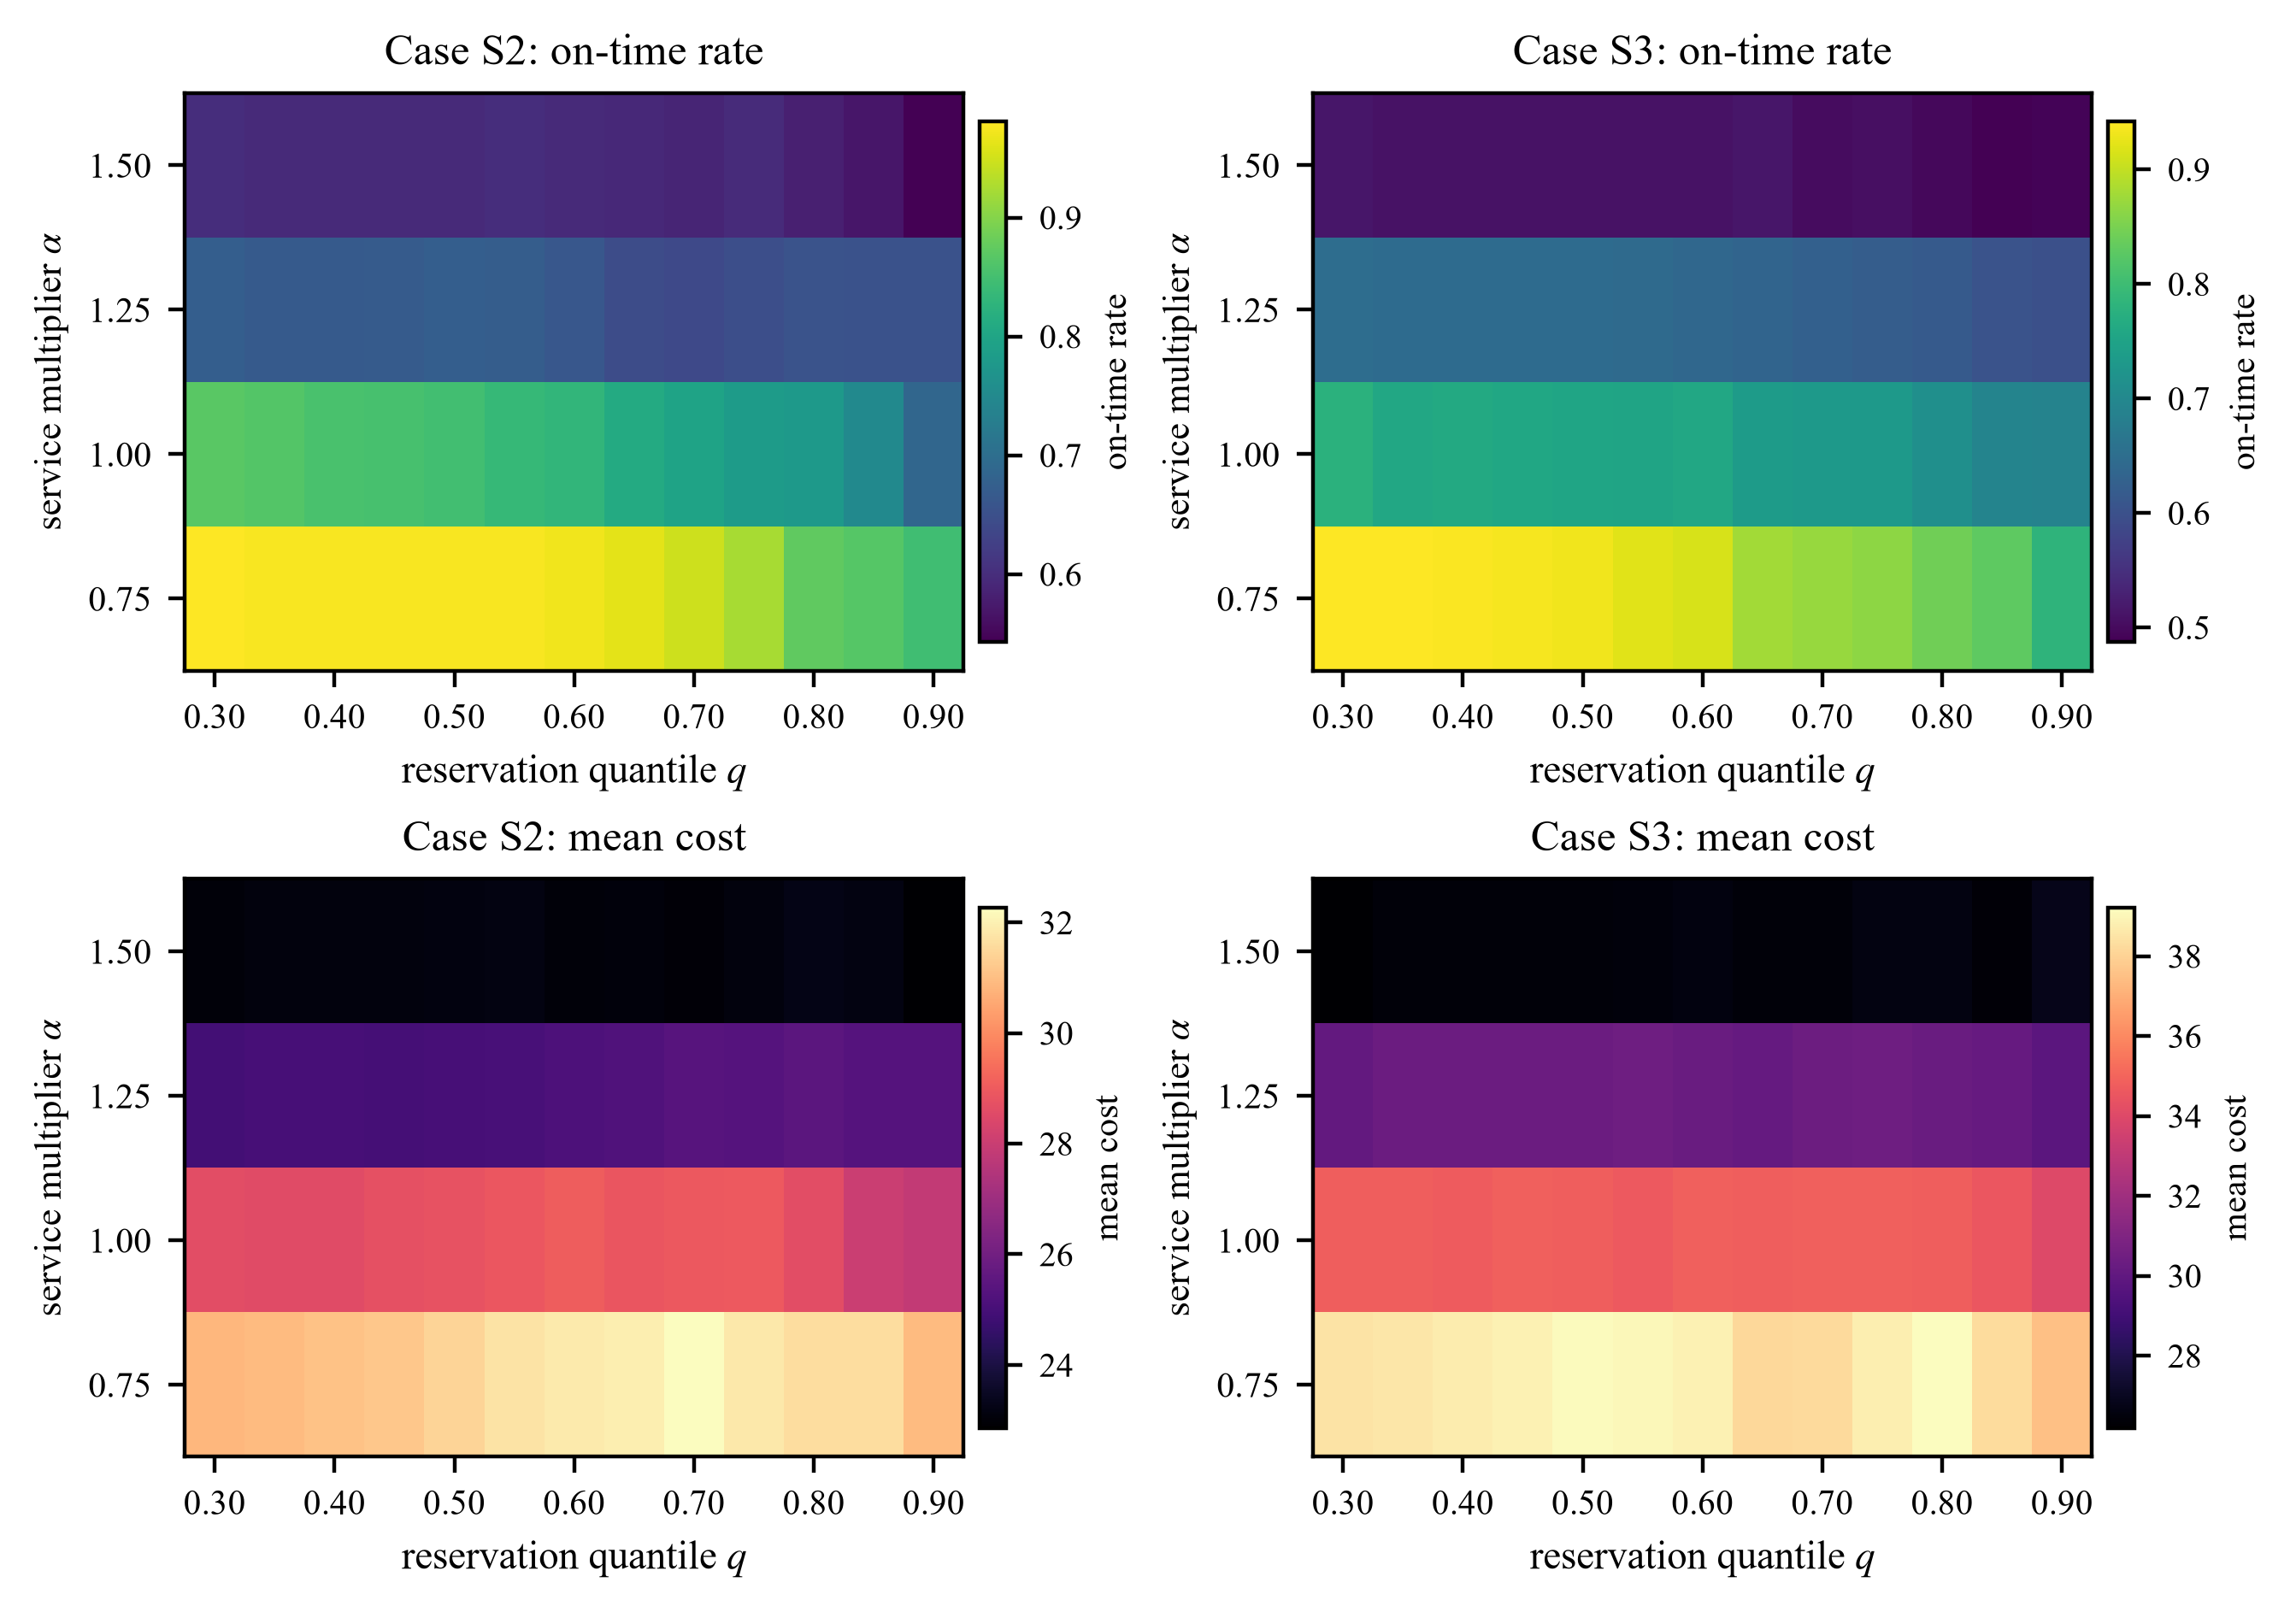
\includegraphics{figures/fig9_phase.png}}
\caption{Phase diagram of the reservation, on the same seeds as the tables. Rows are the
service multiplier, columns the residual quantile; the upper row is the weighted on-time
rate and the lower row the mean cost. The horizontal gradient is small and one-signed, the
vertical gradient is large: the service law moves the rate and the reservation only spends
it.}
\label{fig:phase}
\end{figure}
% numerals-ok: end
